\subsection{\emph{RTAB-Map Node}}
\label{subsec:rtabmapnode}

\emph{RTAB-Map node} merupakan \emph{behavior node} yang digunakan untuk melakukan pemetaan dan lokalisasi menggunakan metode SLAM.
\emph{Node} yang digunakan ini merupakan program \lstinline{rtabmap} yang berasal dari \emph{package} \lstinline{rtabmap_ros}.
\emph{Package} tersebut sendiri merupakan \emph{wrapper} untuk ROS dari \emph{library} RTAB-Map,
  sebuah library SLAM untuk kamera RGB-D, kamera stereo, dan sensor \emph{lidar} berbasis \emph{loop closure detector} \citep{cit:labbe2019}.

\begin{figure}[ht]
  \centering
  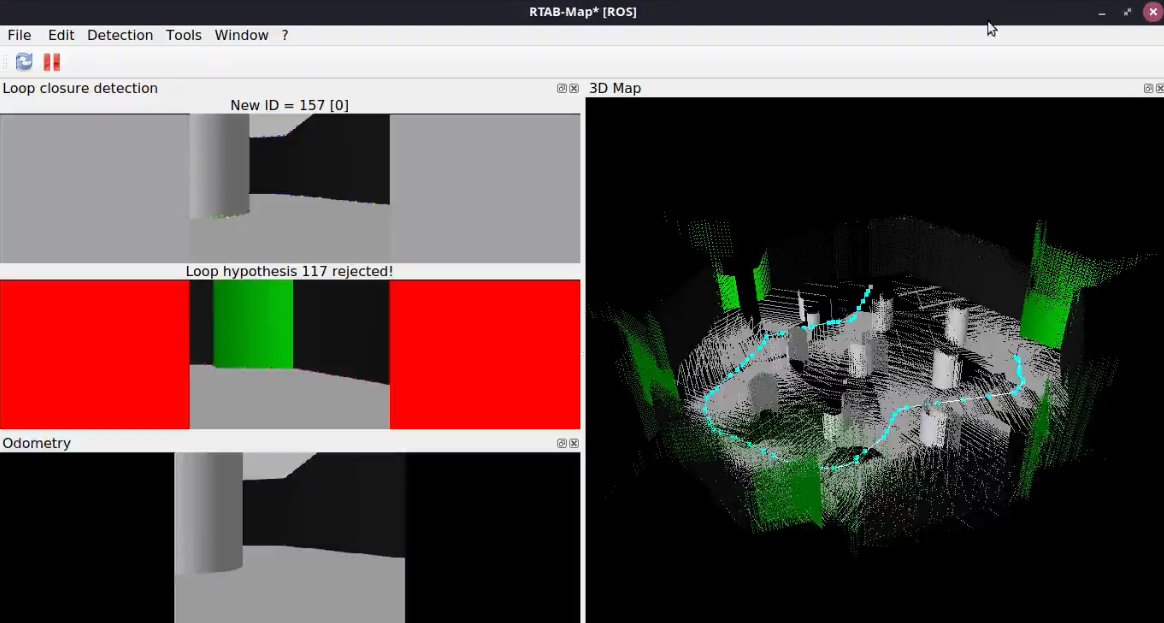
\includegraphics[width=0.9\textwidth,keepaspectratio]{gambar/tampilan-rtabmap.png}
  \caption{Tampilan GUI dari \emph{RTAB-Map node}.}
  \label{fig:tampilanrtabmap}
\end{figure}

Dalam melakukan pemetaan dan lokalisasi,
  \emph{node} ini akan menerima data citra berwarna,
  data citra kedalaman (\emph{depth image}),
  data informasi kamera,
  dan data odometri.
Kemudian data yang diterima tersebut akan diproses menggunakan metode yang ada pada \emph{library} RTAB-Map,
  dan kemudian akan menghasilkan peta lingkungan dalam bentuk 3D serta hasil perkiraan lokalisasi.
Seperti yang terlihat pada gambar \ref{fig:tampilanrtabmap},
  \emph{node} ini memiliki tampilan GUI yang menampilkan data citra berwarna dan citra kedalaman,
  peta 3D yang dihasilkan dalam bentuk \emph{point cloud},
  serta lintasan dari posisi yang telah dilalui berdasarkan data odometri yang diterima.
